%!TEX root = ../main.tex

\chapter{Finding Unreachable Code Using an SMT-Solver}
\label{cha:finding unreachable code using a smt-solver}

The developed approach uses the control flow graph as a basis, but does not transform it into single static assignment form.
During analysis the control flow graph will be traversed and interpreted until every possible execution path was followed and analyzed.
After each interpretation state (e.g., assignments, path conditions) will be added accordingly and must be taken into account.
Merging state has to be handled correctly to make correct statements about the current value of a variable.
The state is represented in the form of a predicate, which may be checked by a system capable of determining satisfiability (e.g., an SMT-solver).
Satisfiable results will continue with the next block(s) and using the new state as a basis and flag this block as visitable.
Unsatisfiable results stop the computation at the current block and will not pursue to continue the path.
Therefore this method is pessimistic.
By using this method, every error should be found in theory (as described in Chapter \ref{cha:conclusion}), since every instruction will be handled like during execution. 
This entails barriers such as 
\begin{itemize}
	\item Significant increase in time needed for analysis. 
	\item Possibly exponentially growing expressions to determine satisfiability.
\end{itemize}
These problems lead to greater execution time, which requires the implementation of reactions (e.g., early stopping, assuming values for variables in loops).

\section{Architecture}
The implementation is part of an already developed static code analysis tool \cite{Prahofer_2012}. 
It consists of different parsers, forms of representation and a rule executor. 
As shown in Figure \ref{fig:general architecture} the tool requires IEC source code and a configuration file for the rule executor.
Basically, rules are Java classes which check if the given IEC source code does not violate any conventions or contain bad code smells. 
Some rules collect metrics, such as lines of code, code complexity, nesting level, cohesion and coupling.
Rules get triggered by certain nodes of the abstract syntax tree, like declarations of variables, function calls, arithmetic expression, et cetera.
For analysis the rule executor traverses the abstract syntax tree and triggers the specified rules provided in the configuration file.
Rules may need different representations of these nodes for more sophisticated analysis. 
When rules are not met, violations will be generated. They contain position, causation and the error message. Violations are written to an XML file, which can be imported to Sonarqube\cite{sonarqube}.


The detection of unreachable code will be implemented in form of a rule as seen in Figure \ref{fig:unreachable-architecture-overview}, the next Section \ref{sec:translation} covers the translation from the abstract syntax tree to a general control flow graph. 
Afterwards the instructions within the control flow graph will be transformed as described in Section \ref{subsec:translate instructions}.
The analysis is covered in Section \ref{sec:analysis}.

\begin{figure}
	\centering
	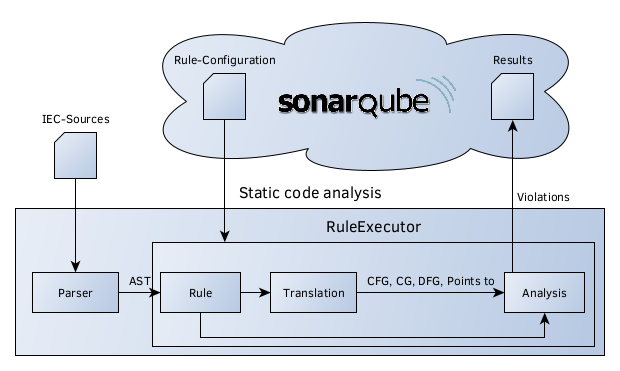
\includegraphics[width=1\textwidth]{static-code-analysis}
	\caption{Architectural overview of the static code analysis tool for IEC source code. After parsing IEC source code, the AST will be passed to the RuleExecutor, which triggers only the configured rules. For more advanced analysis, the AST may be transformed into a different representation. When the source code does not conform to the rules violations will be generated, which can be integrated with Sonarqube.}
	\label{fig:general architecture}
\end{figure}

\begin{figure}
	\centering
	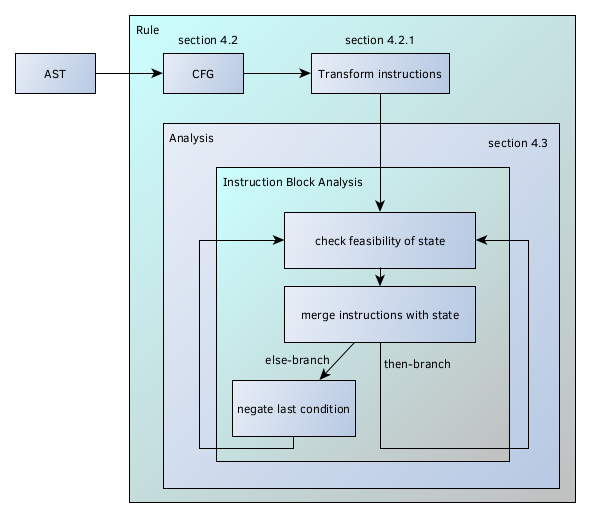
\includegraphics[width=1\textwidth]{unreachable-architecture-overview}
	\caption{General overview of the implementation of the unreachable code detection rule. Each step is annotated in which section it is described. }
	\label{fig:unreachable-architecture-overview}
\end{figure}

\section{Translation of Functions}
\label{sec:translation}
For every function the control flow graph will be calculated and used as the basis. 
Consider the concrete example show in Figure \ref{code:transformation example} as input. 
After parsing the abstract syntax tree will be generated and then used to build the control flow graph (demonstrated in Figure \ref{fig:ast to cfg}).
Information about parameters and global-/system variables also need to be provided in order to handle function-/procedure calls. 
Two separate procedures will be performed on this control flow graph.
\begin{enumerate}
	\item \emph{Unreachable code due to unconditional jumps} is easy to find after the control flow graph was created. Every block (except the beginning block) which does not have any incoming edges must be unreachable.
	Note that these types of errors may also be found as described in Section \ref{sec:analysis}, but were filtered out before.
	\item \emph{Unreachable code due to infeasible conditions} needs a sophisticated and more expensive (in terms of computing resources) approach to identify. The following Section \ref{sec:analysis} describes how to detect them.
\end{enumerate}

\begin{program}
	\begin{GenericCode}
$x$ $\leftarrow$ 3
$y$ $\leftarrow$ 0
		
if $x$ > 2 then
	$y$ $\leftarrow$ $x$ + 1
else
	$y$ $\leftarrow$ $x$ - 1
end
		
while $y$ < $x$ + 10 do
	$y$ $\leftarrow$ $y$ + 1
end
		
log($\downarrow$ $x$)\end{GenericCode}
	\caption{Example containing assignments, branches, loops and procedure-calls. }
	\label{code:transformation example}
\end{program}

\begin{figure}
	\centering
	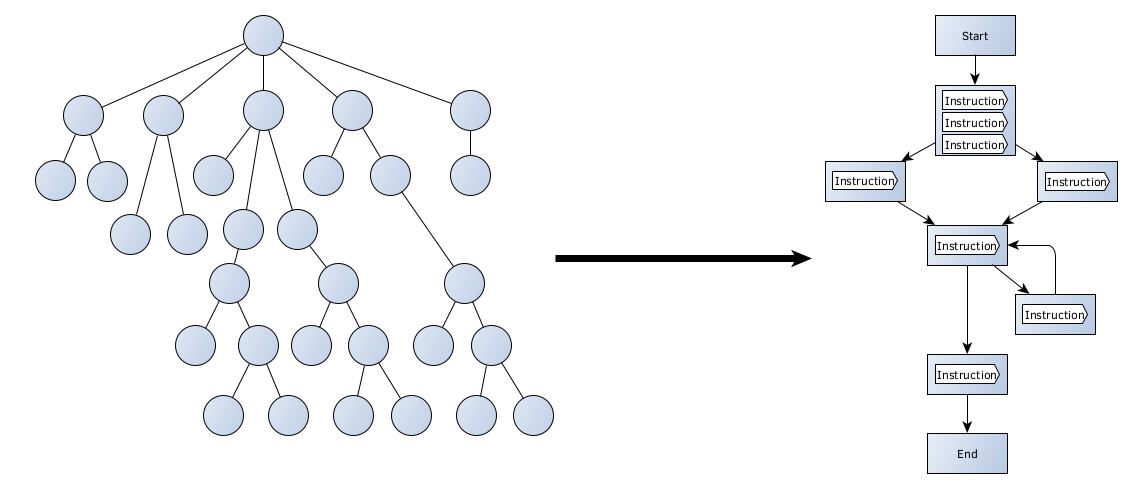
\includegraphics[width=1\textwidth]{ast-to-cfg}
	\caption{In the first step, the abstract syntax tree of a function in listing \ref{code:transformation example} will be translated into the control flow graph.}
	\label{fig:ast to cfg}
\end{figure}


\subsection{Translation of Instructions}
\label{subsec:translate instructions}
The structure of the control flow graph is only one of the necessary components. 
Simplifying instructions makes the overall analysis easier, since each type must be handled differently.
The internal structure of instructions will also be simplified into an AST like structure (see Figure \ref{fig:cfg to internal}). 
Note that the previous control flow graph also contained instructions, which simply were references to nodes in the original AST. 
The new representation contains only the necessary information, which was decoupled from the original AST.

Instructions come in three different types (shown in Figure \ref{fig:state}) and must be marked accordingly:
\begin{enumerate}
	\item \emph{Assignments} are usually the most common form of instructions. They denote a change of the underlying value of a variable and therefore update the state (of said variable) during analysis. 
	\item \emph{Conditions} occur only as the last instruction of a block from a \emph{Controlflow graph}. Note that the last instruction does not necessarily have to be a \emph{condition}.
	\item \emph{Procedure calls} may be mutable and could change variables if they are applied as \emph{output parameters}. % Procedure calls will be dissolved into \emph{assignments} during analysis.
	For intraprocedural analysis of procedures, output parameters will be dissolved into assignments to simplify the process. Basically, it is assumed that out parameters get an undetermined value assigned, which consequently update the state of the variable and may contain any possible value (restricted only by the datatype).
\end{enumerate}
\begin{figure}
	\centering
	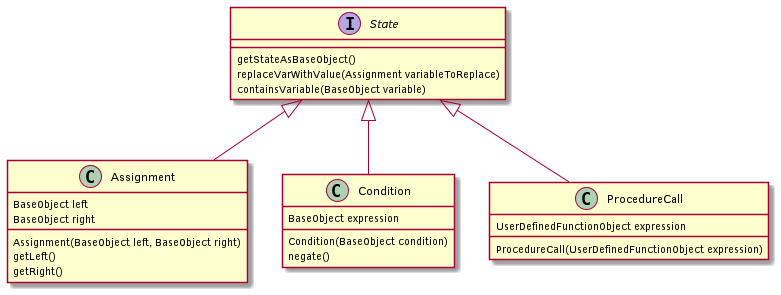
\includegraphics[width=0.85\textwidth]{State}
	\caption{Each instruction in any program may be either represented as an \emph{Assignment}, \emph{Condition} or \emph{ProcedureCall} which encapsulates the expression of types described in Figure \ref{fig:smtobject}. Instructions are processed into a \emph{BaseObject} during evaluation. \emph{Conditions} and \emph{ProcedureCalls} simply contain the expression, whereas \emph{Assignments} separate the left side (the receiving variable) and its concrete value on the right side.}
	\label{fig:state}
\end{figure}
\begin{figure}
	\centering
	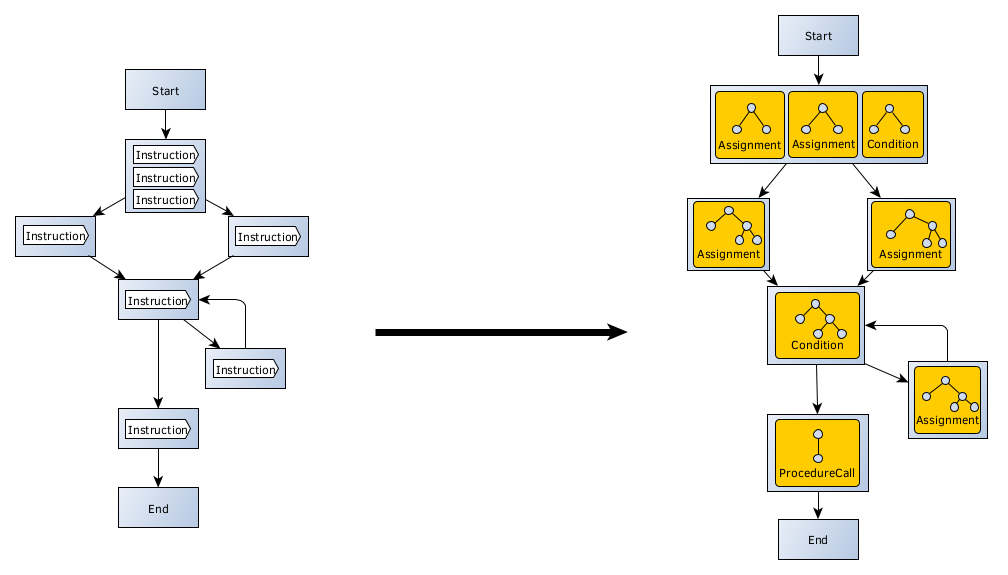
\includegraphics[width=1\textwidth]{cfg-to-internal}
	\caption{The instructions contained in the control flow graph (created before as described in Figure \ref{fig:ast to cfg}) change their representation into a simpler form. As demonstrated in Figure \ref{fig:state} all instructions are either assignments, conditions or procedure calls. Furthermore the concrete instructions are also represented simpler as described in Figure \ref{fig:smtobject}. }
	\label{fig:cfg to internal}
\end{figure}

% AST-Object representation of instructions
Every instruction will also be represented in an AST-like notation as shown in Figure \ref{fig:smtobject}. Each symbol, for example a variable, name of a function or any given literal (such as numbers and strings), are represented as a \emph{BaseObject}. Functions are, in fact, just a special form of this \emph{BaseObject}, which may contain variables. Functions are not only direct function-/procedure calls, but also operations (like + and -). User-defined functions will also be represented as a special form of the described \emph{FunctionObject} before, which contain the declaration of parameters (since named parameters are a language feature of IEC and therefore must be handled correctly), which will be represented as \emph{BaseObjects}. 
This kind of representation makes it easy to work with, since it is a very easy, tree-like data structure which may be traversed easily. Not only replacing variables and values may be done effortlessly, but also the generation of \emph{SMT-Lib} code, since this representation is similar to \emph{LISP}.

\begin{figure}
	\centering
	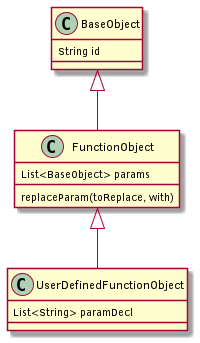
\includegraphics[width=0.2\textwidth]{SMTObject}
	\caption{\emph{AST}-like representation of instructions. }
	\label{fig:smtobject}
\end{figure}
\section{Analysis}
\label{sec:analysis}
After the translation of all functions and instructions the analysis begins. As mentioned in the introduction of this chapter the control flow graph of every function (and procedure) will be traversed. The analysis begins at the single begin block of the graph and ends when all feasible paths reached the exit block. Instruction blocks will be evaluated in order - the same as a program would execute them. 
For each instruction block the instructions will be evaluated. The resulting state must be carried along the analysis and merged correctly to assure valid results. At the end of an instruction block an SMT-solver is used to determine if the current state is feasible or not. Infeasible state may be reached by a combination of conditions. If the current state is infeasible, the \emph{next} block must be unreachable, since the condition at the end of an instruction block determines which branch the flow follows. 
For the determination, if the current state is feasible or not, the SMT-solver Z3 \cite{demouraZ3EfficientSMT2008} is used. The state will be simply translated into the universal, standardized, LISP-like SMT-Lib language \ref{code:translation} which most of the common SMT-solvers are able to interpret. 
If an instruction block is reachable (at least on one occasion), it will be marked as reachable. At the end of the analysis all remaining instruction blocks are marked unreachable.

\begin{program}
	\begin{GenericCode}
procedure $mergeState$($\downarrow$ $instruction$, $\updownarrow$ $state$) begin
	if $instruction.isCondition()$ then
		$state.add($$\downarrow$ $instruction$$)$
	else if $instruction.isAssignment()$ then
		// replace all occurences of variables with their concrete values
		// from the provided $states$ variable
		$replaceVariables($$\updownarrow$ $instruction$, $\downarrow$ $state$$)$ 
		// remove old state e.g. former Assignments and Conditions, which are not
		// valid anymore
		$removeAllOccurrences($$\updownarrow$ $state$, $\downarrow$ $instruction$$)$
		// add the new instruction to the state
		$state.add($$\downarrow$ $instruction$$)$
	end 
end	\end{GenericCode}
	\caption{Merges the new instruction into the existing state. While conditions simply may be added, assignments alter the state, since the concrete value changes and former state can no longer be associated with this variable. }
\label{code:merge state}
\end{program}
\begin{program}
	\begin{GenericCode}
function $solve$($\downarrow$ $state$) begin
	// translate state to SMT-String and pass to Z3
	return $Z3.solve($$\downarrow$ $state.toSMTString())$
end\end{GenericCode}
	\caption{The form (see figure \ref{fig:smtobject}) all instructions are represented in makes the generation of SMTLib code easy. The string containing SMTLib code will simply be passed to the solver directly.}
\label{code:z3 solver}
\end{program}
\begin{program}
	\begin{GenericCode}
procedure $resolveFunctionCalls$($\downarrow$ $instruction$, $\updownarrow$ $state$) begin
	// intra-procedural aprroach:
	// simply remove all variables, which may change.
	$outParams$ $\leftarrow$ $instructions.getOutParams()$
	$state.removeState($$\downarrow$ $outParams$$)$
end	\end{GenericCode}
	\caption{Function calls will be handled in an intra-procedural manner. This is simply realized by just removing any state containing a variable which may change and will be handled like an assignment, whereas the new value is unknown. }
	\label{code:intraprocedural analysis}
\end{program}
\begin{program}
	\begin{GenericCode}
procedure $analyze$ ($\downarrow$ $instructionBlock$, $\downarrow$ $oldState$) begin
	$newState$ $\leftarrow$ $oldState$
	$instructions$ $\leftarrow$ $instructionBlock.getInstructions()$
	$feasible$ $\leftarrow$ $solve(\downarrow oldState)$
		
	if $feasible$ then
		// This instruction block is marked as visitable
		$markInstructionBlock(\downarrow instructionBlock)$ 
		for $instruction$ in $instructions$ do
			$resolveFunctionCalls$($\downarrow$ $instruction$, $\updownarrow$ $newState$)	
			if not $instruction.containsFunctionCall()$ then
				// Functioncalls were already handled at this point
				$mergeState$($\downarrow$ $instruction$, $\updownarrow$ $newState$)
			end 
		end
		$analyze$($\downarrow$ $instructionBlock.getThenBranch()$, $\downarrow$ $newState$)
		// By following the else-branches last instruction, if it was a condition, must be negated
		$analyze$($\downarrow$ $instructionBlock.getElseBranch()$,$\downarrow$ $newState.negateLastInstruction()$)
	end
end	\end{GenericCode}

	\caption{The main component of the unreachable code detection is the analysis of instruction blocks. Beginning with no state set it will be added subsequently by traversing the control flow graph and adding accumulated state. 
	At first the current state must be checked for feasibility. Only if it is feasible (see Listing \ref{code:z3 solver}) this the instruction block can be marked as reachable and new instructions may be added to the state as described in Listing \ref{code:merge state} and Listing \ref{code:intraprocedural analysis}.	
	Afterwards the possible branches will be followed (a maximum of two) containing the new assembled state.}
	\label{code:instruction block analyzer}
\end{program}

% TODO: add example for translation
\begin{program}
	\begin{GenericCode}
$i$ $\leftarrow$ 1
$x$ $\leftarrow$ 5
if $i$ < $x$ then 
	// ...
end\end{GenericCode}
	\begin{GenericCode}
;; Check if condition evaluates TRUE
(declare-fun x () Real)
(declare-fun i () Real)
(assert (and (= i 1) (= x 5) (< i x)))
(check-sat)
; => SAT\end{GenericCode}
	\begin{GenericCode}
;; Check if condition evaluates FALSE	
(declare-fun x () Real)
(declare-fun i () Real)
(assert (and (= i 1) (= x 5) (not (< i x))))
(check-sat)
; => UNSAT\end{GenericCode}
	\caption{Translation of the IEC-Code. As shown above, each variable must be declared beforehand (therefore the implementation must be aware of the type). The assertion includes the complete state (including assignments and conditions). Conditions are the only part which could lead to an unfeasible result. Every Instruction-Block must contain at least one edge out of the block (with the exception of the exit block), but may also contain a second edge, indicating the path of a condition evaluates false. Therefore the condition must be negated.}
	\label{code:translation}
\end{program}

\subsection{Interpretation of Instructions}
\label{sub:Interpretation of Instructions}
% Handling of and state management
One of the central parts during analysis is the handling of states. Each instruction must have the same effect as it was executed after compilation. 
As described before, states come in three forms: assignment, condition, procedure-/function call, which all must be handled accordingly (see the implementation in Listings \ref{code:intraprocedural analysis} and \ref{code:merge state}): 

\begin{itemize}
	\item Conditions are just added to the state as they are. 
	\item Assignments have to be handled differently. Assignments change the current value of a variable and therefore the path condition is not valid afterwards. It must be reset therefore. 
		If there is any variable on the right side, it must be replaced by its value. Especially cases which contain the same variable on the left and right side must use the values instead of the identifier, since a SMT solver does not contain any mechanism for reassignment, but rather a bidirectional unification. For example the statement (= x (+ x 1)) will always result in an unsatisfiable state.
	\item Procedure-/function-calls will be handled as described in \ref{sub:handling procedure and function calls}. Out parameters and the return values are represented as assignments. 
\end{itemize}

After all instructions are interpreted, it will be translated into SMT-Lib code (see Listing \ref{code:z3 solver}), which tests if the next blocks are available. 
The state will be passed on until unreachable code is detected or the exit block is reached.
The implementation can be viewed in Listing \ref{code:instruction block analyzer}. 

\subsubsection{Examples}
The following examples contain code, control flow graph and also the order in which the algorithm evaluates instruction blocks. These blocks are annotated with the current state and which instruction block is evaluated currently. As described earlier the instructions of the current instruction block take effect in the analysis of the next block. The blue and orange color indicate if the state is statisfiable.


Figure \ref{fig:assignmentOnly} demonstrates how assignments are handled. In the second instruction the variable $x$ gets reassigned using the old value.
As described earlier the variables must always be replaced by their concrete values. The statement (= x (+ x 1)) does not make any sense to a SMT-solver. 
Since this example only contains assignments, every block is reachable.


The example shown in Figure \ref{fig:simpleIf} demonstrates branching when encountering if-then-else statements. After branching potential following instructions will be evaluated for each path separately. 


Figure \ref{fig:simpleLoop} demonstrates how a simple loop will be evaluated. Note that for each iteration the same branching process described before will be applied. 
This is the reason why so many branches will be created, which will have a negative impact on run time.


The last example show in Figure \ref{fig:unconditionalJump} shows an example containing an unconditional jump in a loop. There are no incoming edges into BasicBlock 4, which indicates that these statements of this basic block are unreachable.

\begin{figure}
	\begin{GenericCode}
$x$ $\leftarrow$ 1
$x$ $\leftarrow$ $x$ + 1
$i$ $\leftarrow$ $x$\end{GenericCode}
	\centering
	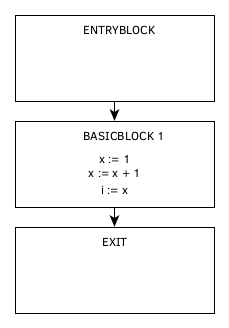
\includegraphics[width=0.3\textwidth]{assignments-only-cfg}
	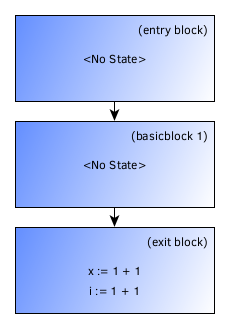
\includegraphics[width=0.3\textwidth]{assignments-only}
	\caption{Demonstration of simple assignments and reassignments. The resulting state is displayed on the next block.}
	\label{fig:assignmentOnly}
\end{figure}

\begin{figure}
	\begin{GenericCode}
if $x$ = 2 then 
	y $\leftarrow$ true
else
	y $\leftarrow$ false
end\end{GenericCode}
	\centering
	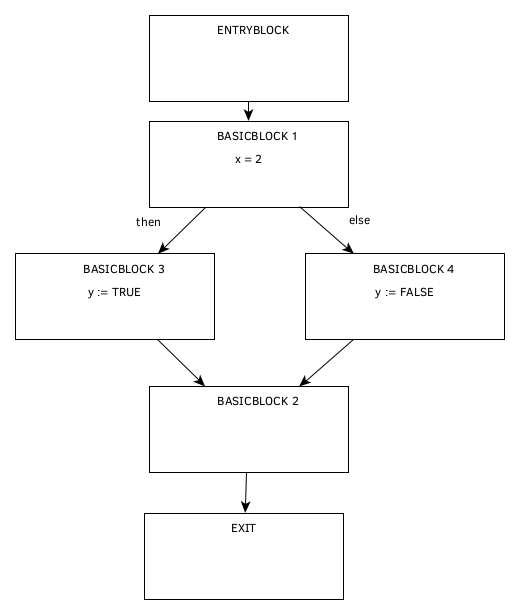
\includegraphics[width=0.4\textwidth]{simple-if-cfg}
	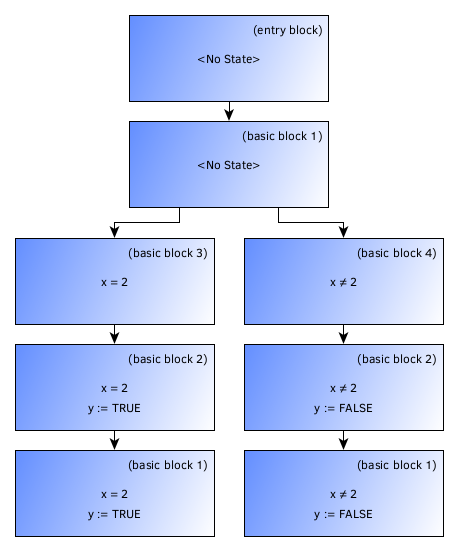
\includegraphics[width=0.4\textwidth]{simple-if}
	\caption{Simple selection (IF). The flow is divided into to branches - the condition could either be TRUE or FALSE. Each path will be evaluated separately. }
	\label{fig:simpleIf}	
\end{figure}

\begin{figure}
	\begin{GenericCode}
for $i$ $\leftarrow$ 0..$x$ do
	$y$ $\leftarrow$ $i$ + $x$
end	\end{GenericCode}
	\centering
	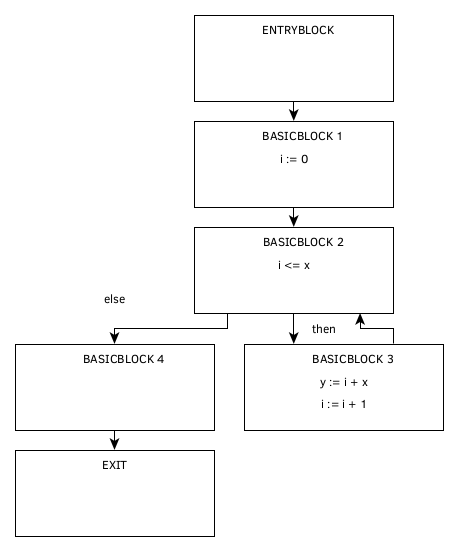
\includegraphics[width=0.4\textwidth]{simple-loop-cfg}
	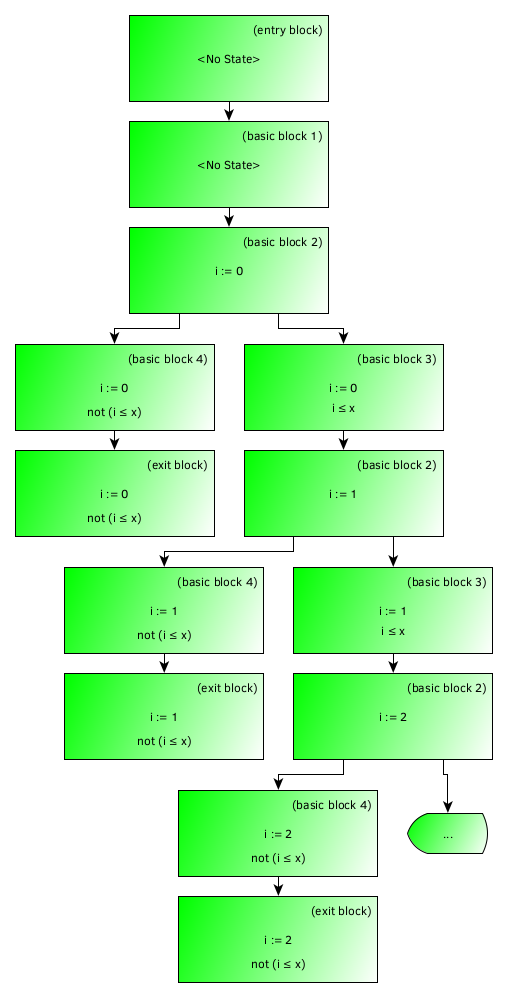
\includegraphics[width=0.4\textwidth]{simple-loop}
	\caption{After each iteration the condition will be evaluated with the new state again. Every node is reachable, even tough the analysis stopped prematurely, since the analysis could eventually be indefinitely. }
	\label{fig:simpleLoop}
\end{figure}

\begin{figure}
	\begin{GenericCode}
$i$ $\leftarrow$ 1
while $i$ < 10 do
	$i$ $\leftarrow$ 2
	break
	$i$ $\leftarrow$ 3
end\end{GenericCode}
	\centering
	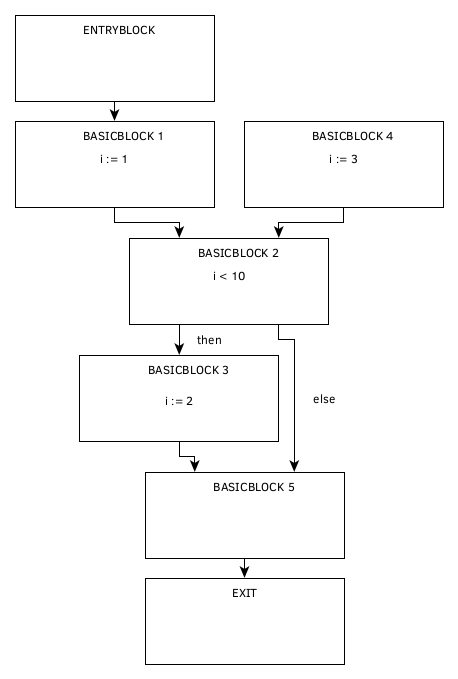
\includegraphics[width=0.4\textwidth]{unconditional-jump-cfg}
	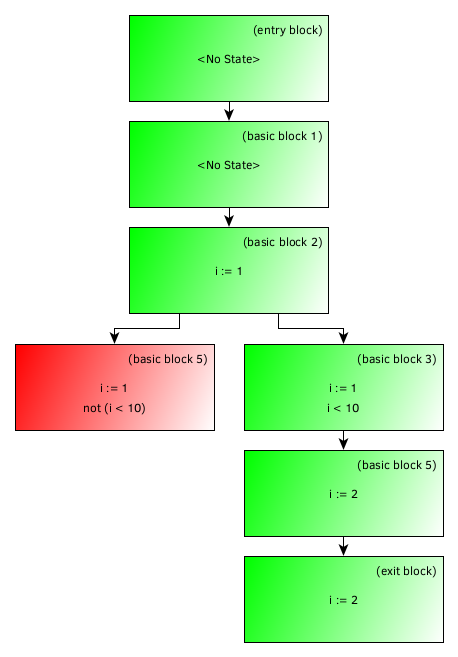
\includegraphics[width=0.4\textwidth]{unconditional-jump}
	\caption{Instruction block 4 is not reachable, since the flow was interrupted by an unconditional jump.}
	\label{fig:unconditionalJump}
\end{figure}

\subsection{Early stopping}
\label{sub:early stopping}
Ideally, there is an infinite amount of time available for the analysis. Realistically this is impossible to accomplish, therefore mechanisms to stop the computation early must be implemented.
Due to possible mutable state it is not easy to determine values without interpreting the flow of the program. 
% This is the main reason the approach \ref{cha:state of the art} does not detect possible unreachable Code in loops \ref{code:ssa-defect}. 
But being able to find this kind of defects comes with greater execution time. Without proper guards the analysis would take an infinite amount of resources and never find a solution.
\begin{itemize}
	\item One of the simplest mechanisms could be, that as soon as every instruction block is marked as reachable, the analysis should stop.
	\item As soon as loops are involved a multitude of different strategies would come to mind. 
	\begin{itemize}
		\item Following the flow of a loop a maximum set amount of time. Note that this approach could lead to false-positives, since the loop only finished partly. 
		\item Stopping the analysis as soon as too many iterations were made. No false positives will be reported, but the analysis is incomplete.
		\item Resetting the state of every assigned variable inside the body of the loop. Therefore no false positives will be reported, but may overlook some instances of unreachable code.
	\end{itemize}
\end{itemize}

\subsection{Handling Procedure and Function calls}
\label{sub:handling procedure and function calls}
Procedure and function calls are handled intraprocedurally, meaning return values are not calculated. That simply means every function call just checks if the declaration contains any (mutable) in and out parameters or is used on the right hand side of an assignment.
Either way said variables must reset their state, since the value may change. 
This approach is definitely lighter on resources (in contrast to interprocedural analysis), but may not be able to detect certain defects which may be obvious to a human. Consider the usage of the identity function. Since the intraprocedural approach does not consider the body of the called function, the state must reset the assigned variable, even tough it does not change.

\subsection{Problems and Barriers}
\label{sub:problems and barriers}
Especially the evaluation of loops is not gentle on resources and processing power. The number of blocks to evaluate grows exponentially. Naturally loops are very common. In theory this approach could find every instance of unreachable code, only limited by available resources. Multiple strategies described before in Section \ref{sub:early stopping} may be applied to reduce the number of iterations.
The consequences of these strategies are, that not every instance of unreachable code can be detected, making this method not necessarily superior to the traditionally implemented approach.
It may be possible to use some sort of preprocessing and potentially make it possible to evaluate loops only once, which could reduce the execution time drastically.
The implementation of such a form of preprocssing must take mutations into account and ideally guarantee the same accuracy.
Without any preprocessing interprocedural analysis of function-/procedure calls may also increase execution time significantly, since they must be interpreted as well. Here also some sort of preprocessing would be interesting. 
Recursive functions (directly and indirectly) would also lead to an increase of execution time.
